\documentclass[12pt]{scrartcl}
\title{Assignment 3\\ Drawing stuff report}
\author{\textbf{Flow Overstack Team}\\ Cesana Filippo\\ Hartmann Kathrin\\ Rodolfo Masera Tommaso\\ Stucchi Jacopo\\ Taillefert Stefano}
\date{}
\setlength{\parindent}{0pt}

\usepackage{graphicx}
\usepackage{float}

\begin{document}
\maketitle

\section{Introduction}

	Write a brief introduction referring back to your project and it basic concepts.

\section{Persona}

	Describe briefly your design persona as distilled from the analysis of data gathered during Contextual Inquiry.

\section{Ideation and sketching}

	Describe your ideation and sketching process and how these two activities fit together.

\section{Workspace and materials}

	Describe your workspace and the materials you used.
	
\section{Photos}

	If appropriate, show photos of your team at work.
	
	%Kathrin's group picture here
	
\section{Sketches}
	
	Show scans of selected sketches.
	
	\begin{figure}[H]
        		\centering
       		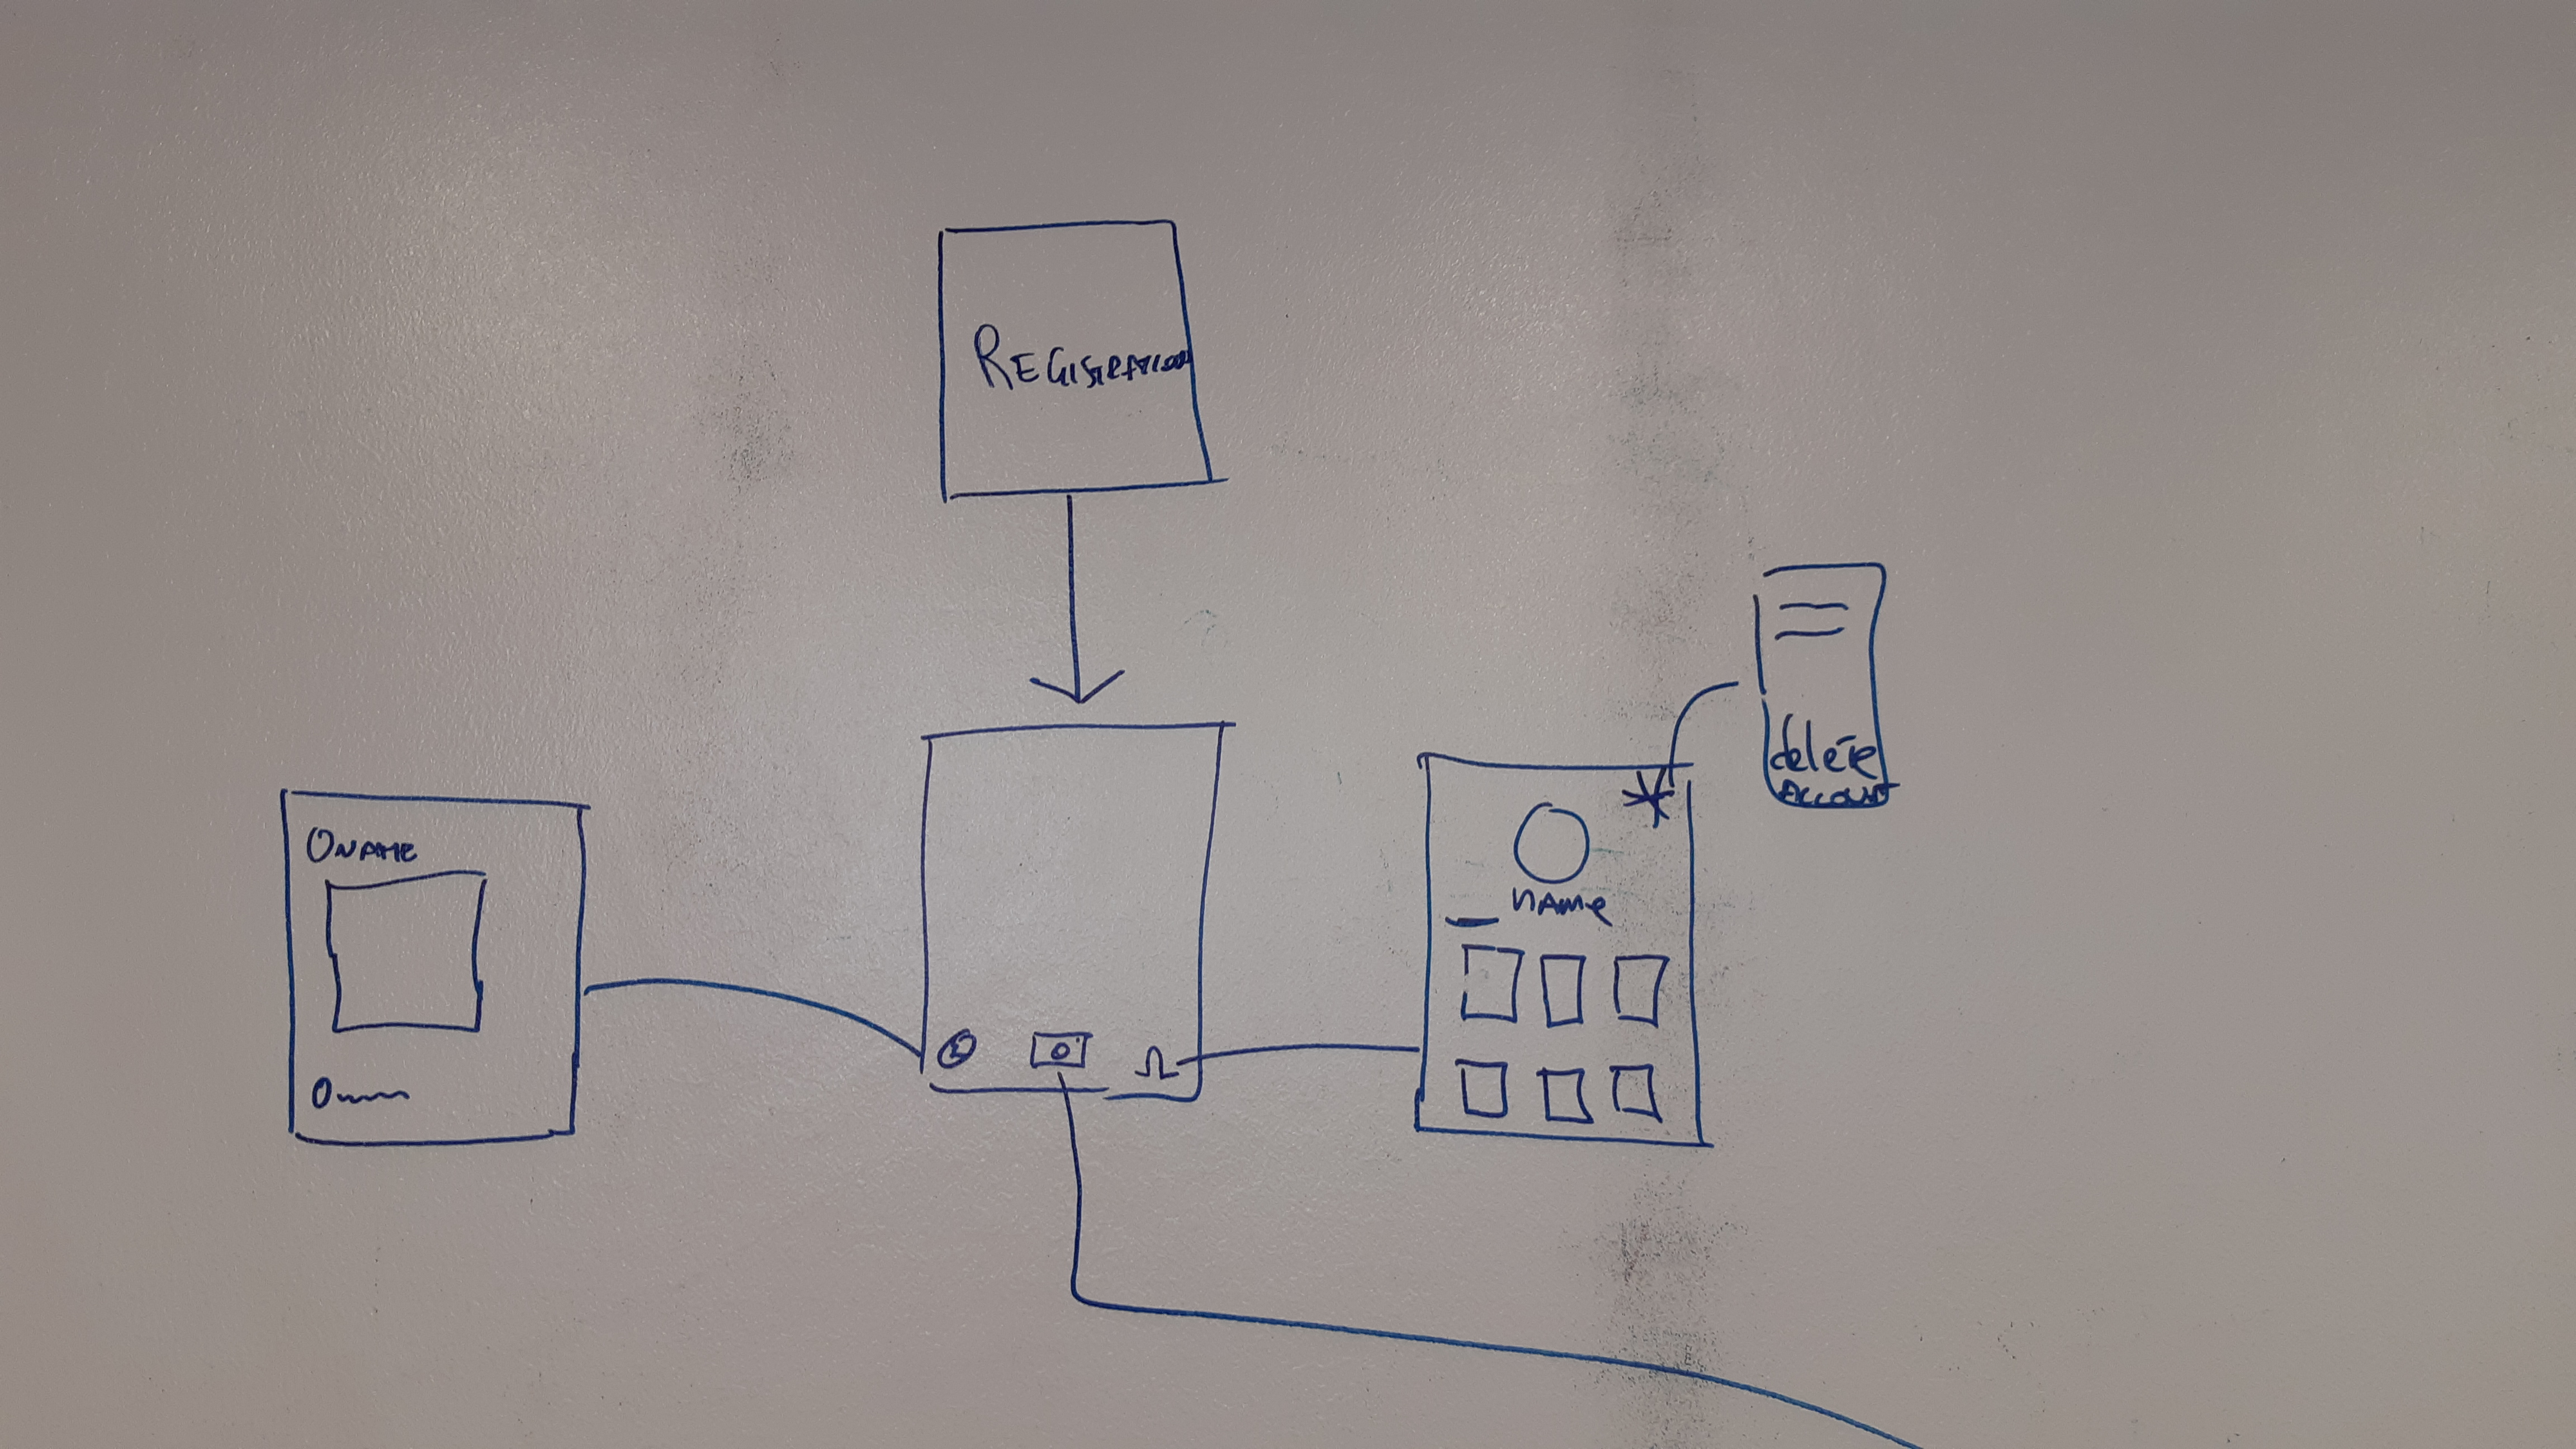
\includegraphics[width=\textwidth]{design1.jpg}
       		\caption{The very first sketch}
        		\label{sketch1}
	\end{figure}
	
\section{Storyboard}
	
	Show your storyboard (probably as scans or photos), and explain the process very briefly. Explain the frame that shows the transition from one adjacent frame to another.
	
	\begin{figure}[H]
        		\centering
       		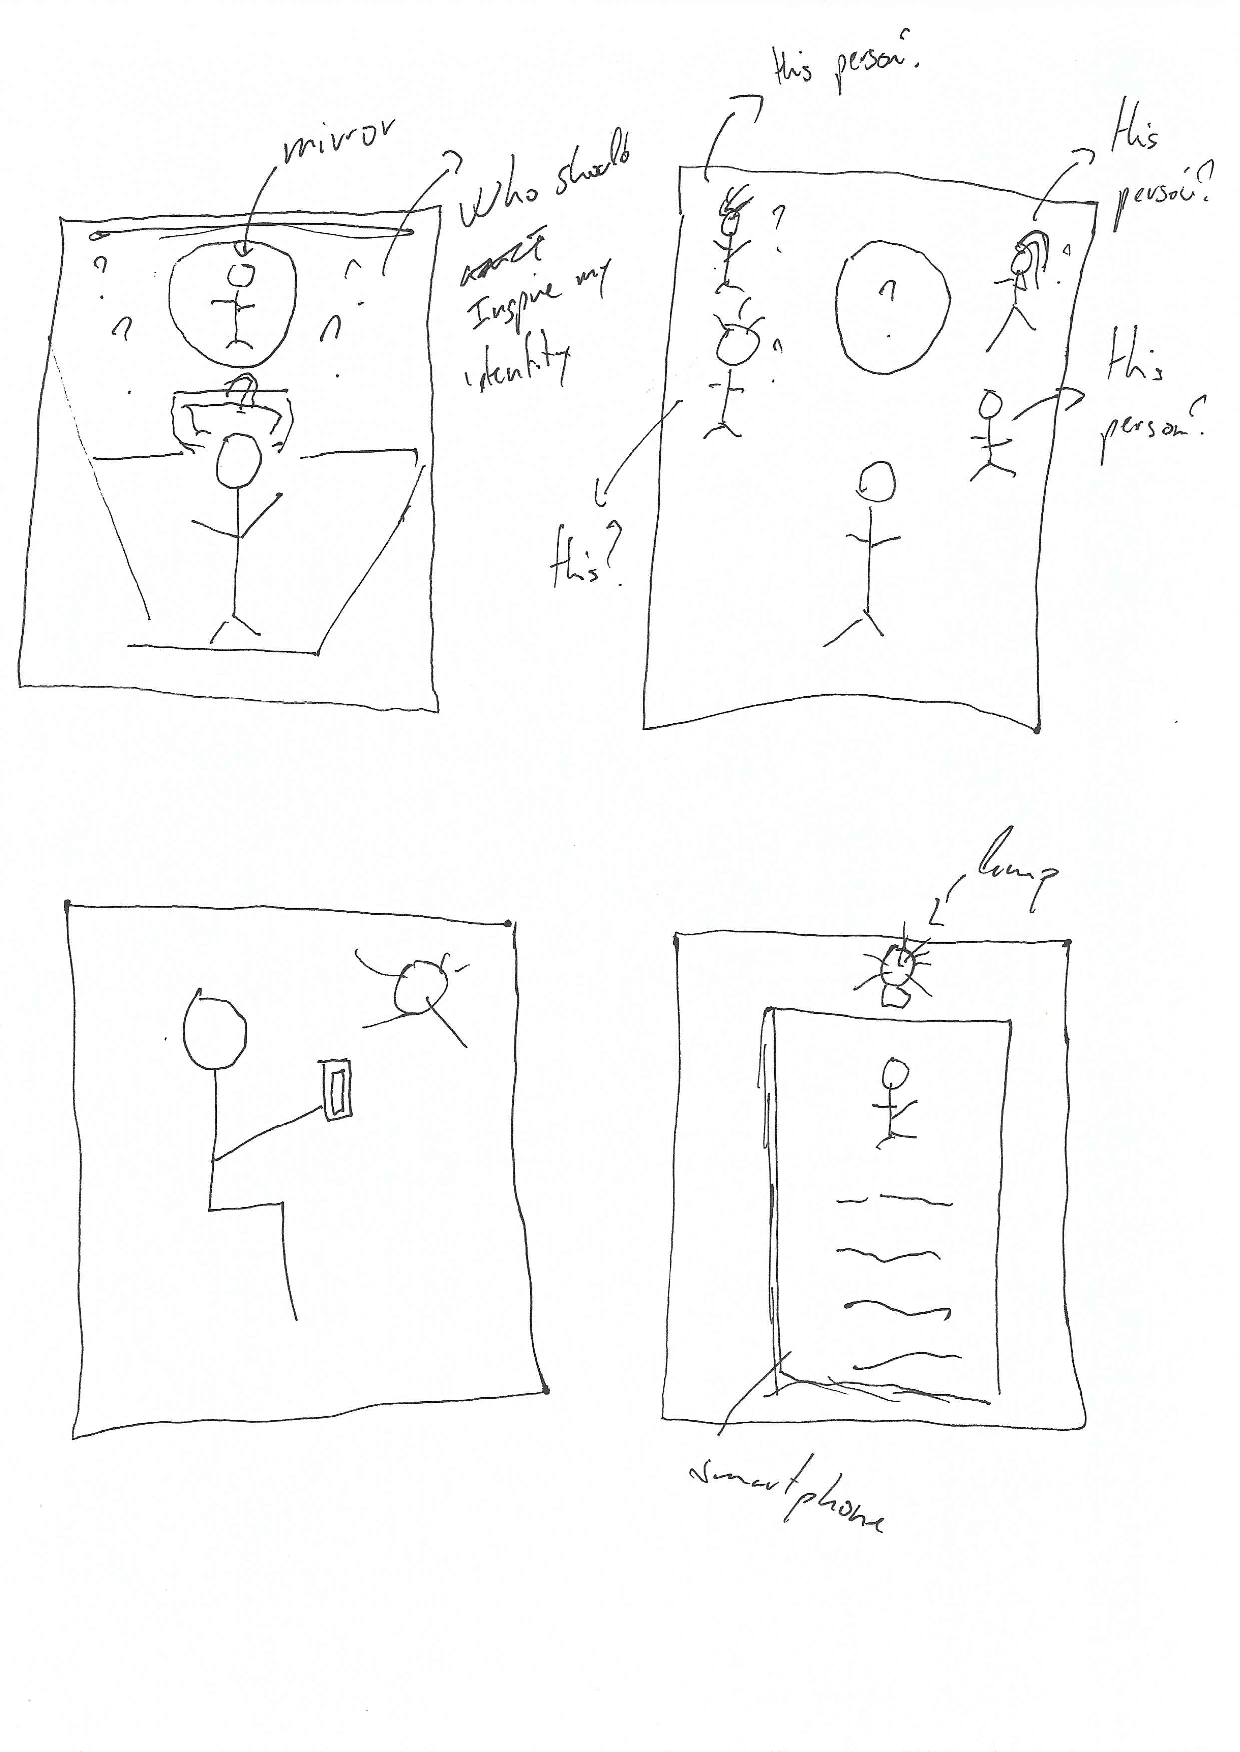
\includegraphics[width=\textwidth]{sketches/story1.pdf}
       		\caption{The First Story (by Filippo)}
        		\label{story1}
	\end{figure}
	
	\begin{figure}[H]
        		\centering
       		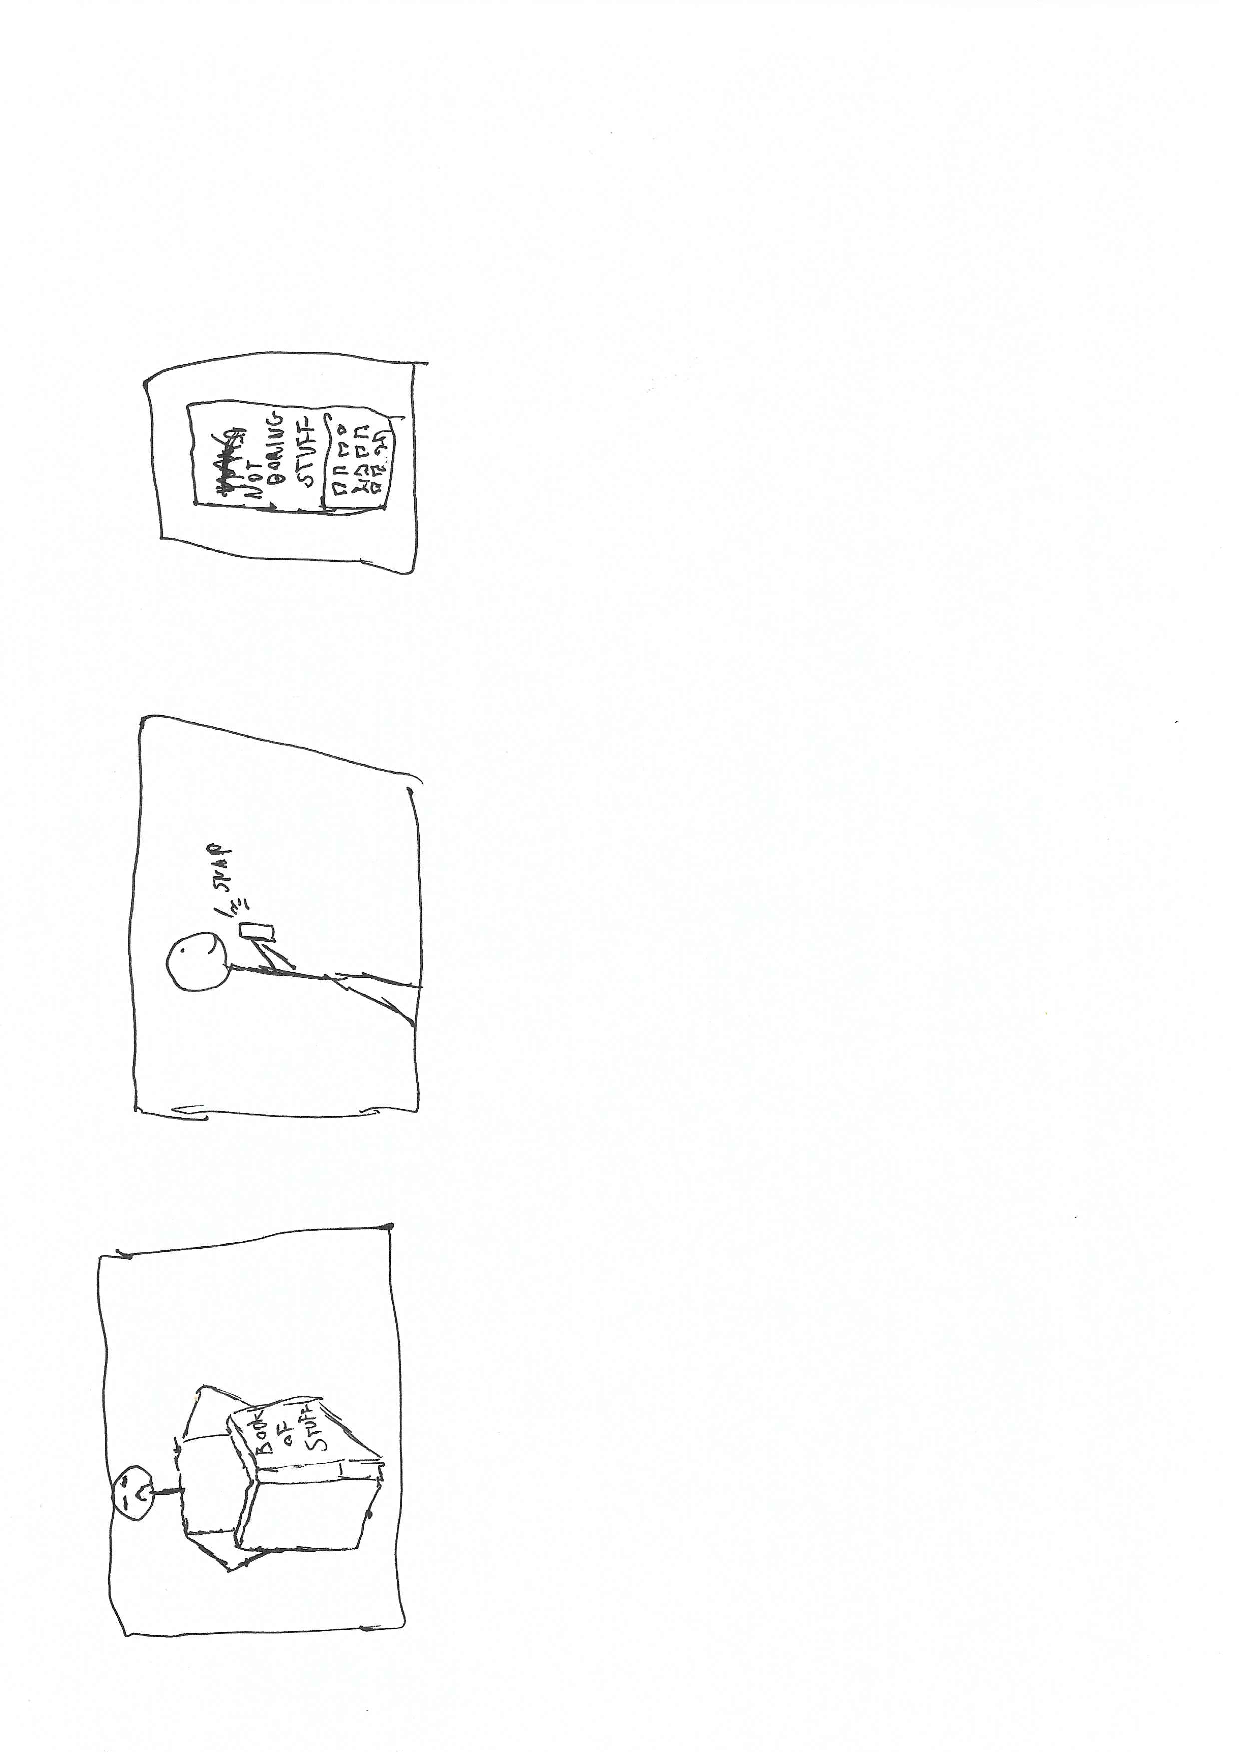
\includegraphics[width=\textwidth]{sketches/story2.pdf}
       		\caption{The Second Story (by Tommaso)}
        		\label{story2}
	\end{figure}
	
	\begin{figure}[H]
        		\centering
       		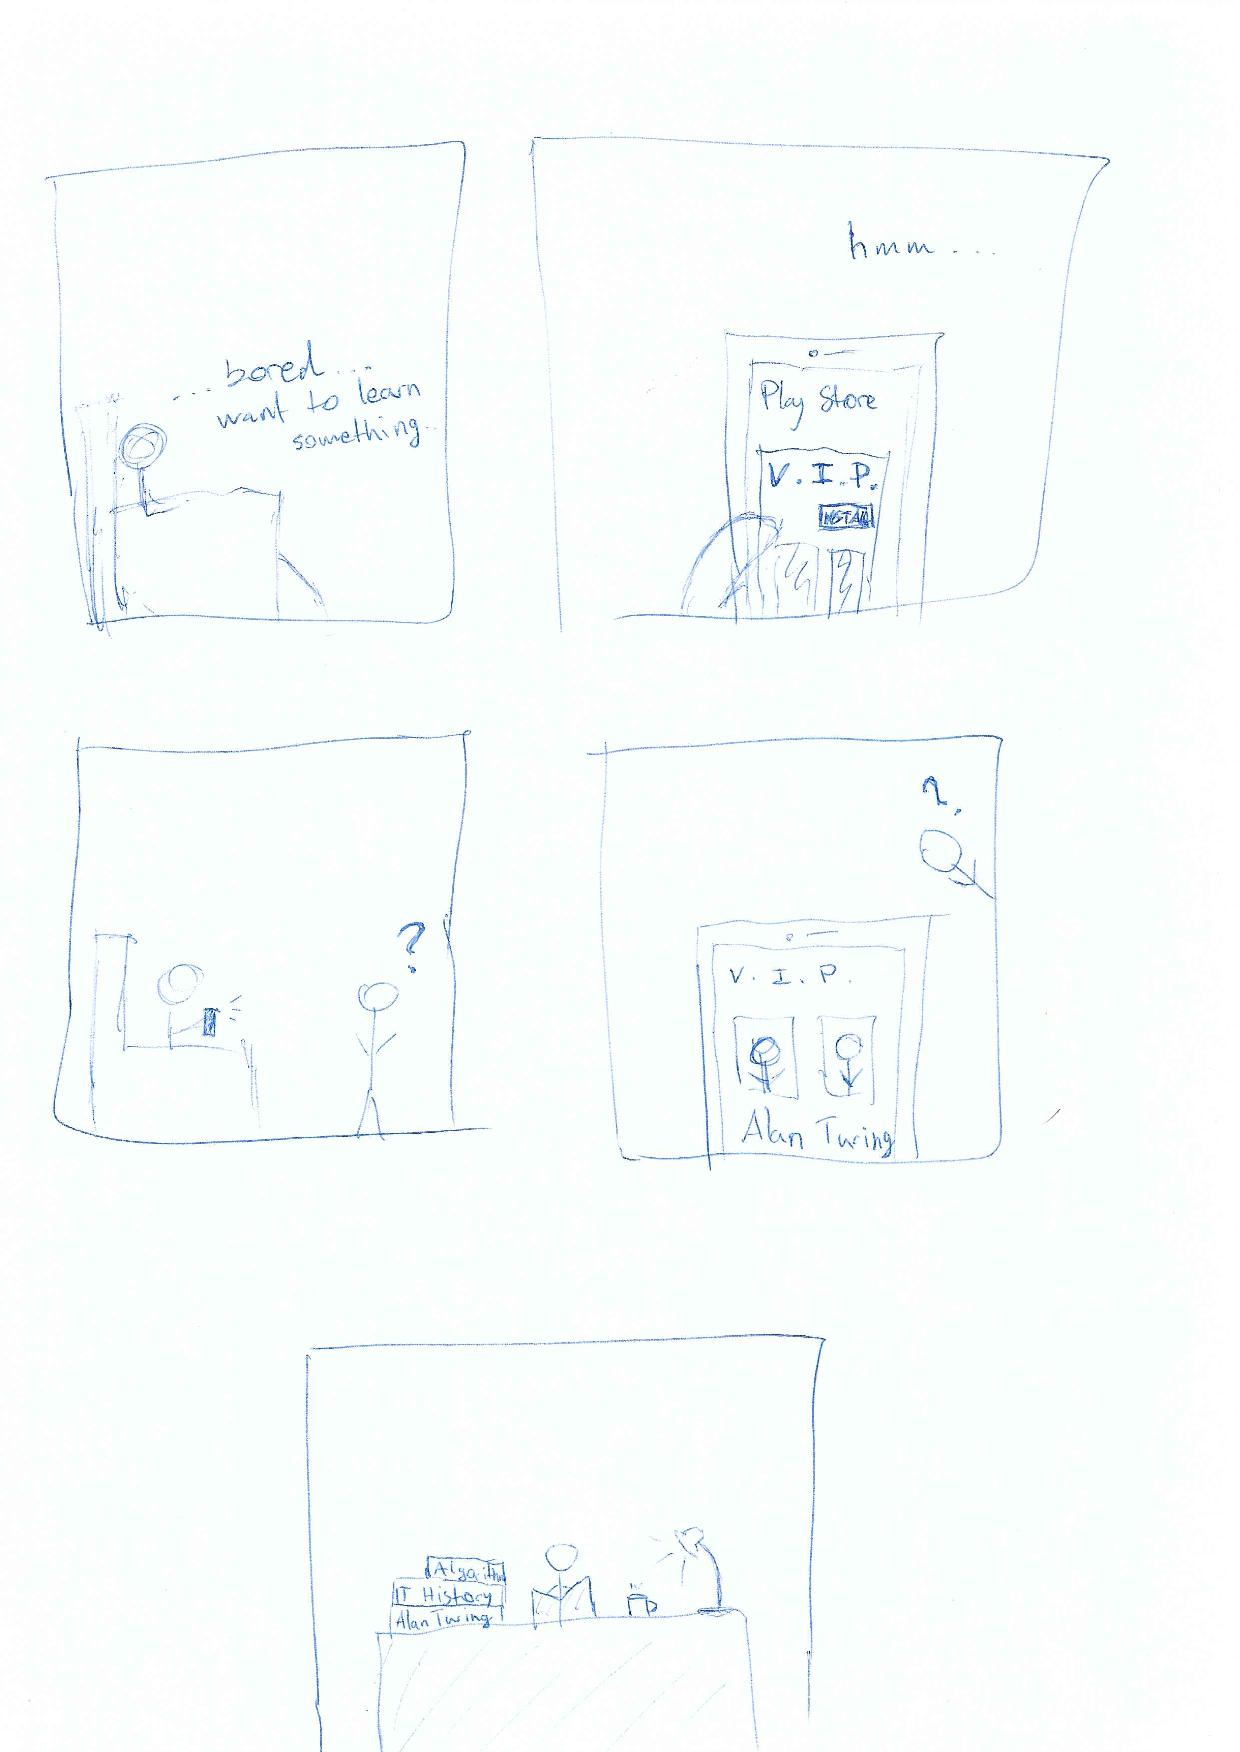
\includegraphics[width=\textwidth]{sketches/story3.pdf}
       		\caption{The Third Story (by Stefano)}
        		\label{story3}
	\end{figure}
	
	%Jacopo' story here

\section{Wireframe}

	Make a wireframe representation of a set of related intermediate screen designs, corresponding to the usage/design scenario you used for the storyboard above.  Show screen layout and navigation.
	
\section{Conclusions}

	Write conclusions about what you have learned and progress in your project.

\end{document}